\resizebox{0.3\textwidth}{!}{%
	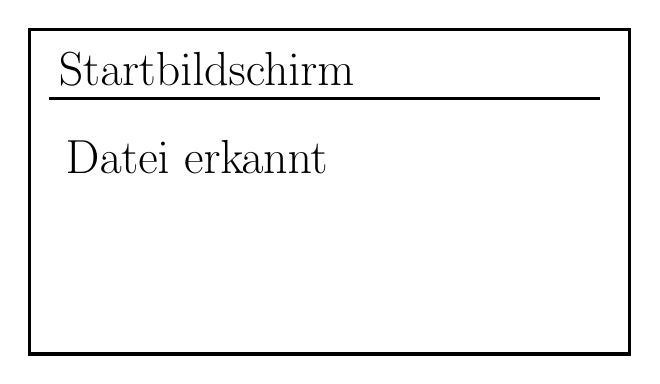
\begin{tikzpicture}
		\tikzstyle{every node}=[font=\fontsize{14.2pt}{18.5pt}\selectfont]
		\draw [fill={rgb,255:red,255; green,255; blue,255}, fill opacity=1, line width=1.2pt] (3.25,16) rectangle (10.875,11.875);
		\draw [line width=1.2pt] (3.5,15.125) -- (10.5,15.125);
		\node [font=\fontsize{18.2pt}{23.7pt}\selectfont, fill={rgb,255:red,255; green,255; blue,255}, fill opacity=1, text opacity=1, inner xsep=0.080cm, inner ysep=0.085cm, rounded corners=0.020cm] at (5.5,15.5) {Startbildschirm};
		\node [font=\fontsize{18.2pt}{23.7pt}\selectfont, fill={rgb,255:red,255; green,255; blue,255}, fill opacity=1, text opacity=1, inner xsep=0.080cm, inner ysep=0.085cm, rounded corners=0.020cm] at (5.375,14.375) {Datei erkannt};
	\end{tikzpicture}
}%